\chapter{Spazi affini}
\section{\(A_n(K)\), spazio affine di dimensione \(n\)}
\dfn{Spazio affine}{Si dice \textbf{spazio affine} di dimensione \(n\) sul campo \(K\), e si indica \(\AA_{n}(K) \), la struttura costituita da
\begin{enumerate}
    \item un insieme non vuoto \(A \), detto insieme dei punti
    \item uno spazio vettoriale \(V_n(K)\) 
    \item un'applicazione \[
    f: \quad A \times A \to V_n(K)
    \] con le seguenti proprietà
    \begin{enumerate}
        \item \(\forall P \in A \ e \ \forall v \in V \quad \exists ! \ Q \in A : \quad f(P, Q) = \vec{PQ} = v\)
        \item \(\vec{PQ} + \vec{QR} = \vec{PR} \quad \forall P, Q, R \in A\)
    \end{enumerate}
\end{enumerate}}

\mprop{}{In \(A_n(K)\), per ogni \(P,Q\) e \(R \in A\)
\begin{enumerate}
    \item il vettore \(\vec{RR} = \ul{0} \)
    \item \(\vec{PQ} = \vec{PR} \iff Q = R\)
    \item \(\vec{PQ} = \ul{0}  \iff P=Q\)
    \item \(v = \vec{PQ} \implies -v = \vec{QP}\)
    \item \(\forall P_1, P_2, Q_1, Q_2 \in A\) risulta \(\vec{P_1P_2} = \vec{Q_1Q_2} \iff \vec{P_1Q_1} = \vec{P_2Q_2}\)
\end{enumerate}}

\pf{Dimostrazione}{ Dimostriamo ogni punto separatamente
\begin{enumerate}
    \item \(\vec{R R} + \vec{RR} = \vec{RR}\) perciò \(2 \vec{RR} = \vec{RR} \iff \vec{RR} = \ul{0} \)
    \item posto \(v = \vec{PQ}\) allora \(v = \vec{PR}\), ma \(\exists ! \ Q : \ \vec{PQ}=v \implies R = Q\) 
    \item per la proprietà 1 \(\vec{RR} = \ul{0} \implies \) per l'unicità di \(Q: \vec{PQ}=\ul{0} \implies Q=P\)
    \item \(\vec{PQ} + \vec{QP} = \vec{PP} = \ul{0} \implies \vec{PQ} = - \vec{QP}\)
    \item ovvio, essendo \(\vec{P_1P_2} + \vec{P_2Q_2} = \vec{P_1Q_2} = \vec{P_1Q_1} + \vec{Q_1Q_2}\)
        \begin{center}
            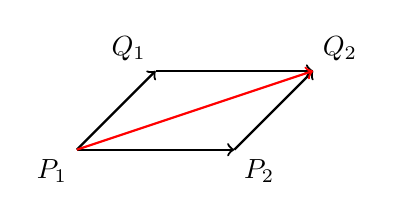
\begin{tikzpicture}
                \coordinate (P_1) at (0, 0);
                \coordinate (P_2) at (2, 0);
                \coordinate (Q_1) at (1, 1);
                \coordinate (Q_2) at (3, 1);
                \draw[thick, ->] (P_1) -- (P_2);
                \draw[thick, ->] (P_1) -- (Q_1);
                \draw[thick, ->] (Q_1) -- (Q_2);
                \draw[thick, ->] (P_2) -- (Q_2);
                \draw[red, thick, ->] (P_1) -- (Q_2);
                \node[below left] at (P_1) {\(P_1\)};
                \node[below right] at (P_2) {\(P_2\)};
                \node[above right] at (Q_2) {\(Q_2\)};
                \node[above left] at (Q_1) {\(Q_1\)};
            \end{tikzpicture}
        \end{center} 
\end{enumerate}
}

\dfn{Sottospazio affine}{Sia \(A_n(K)\) uno spazio affine. Si dice \textbf{sottospazio affine} di dimensione \(m \le n\) una struttura data da
\begin{enumerate}
    \item \(\emptyset \neq A' \subseteq A\), detto \textbf{sostegno del sottospazio affine} 
    \item \(V_m(K)\) sottospazio di \(V_n(K)\) 
    \item la restrizione dell'applicazione \(f\) ad \(A' \times A'\) troncata a \(V_m(K)\), purché questa sia ancora un'applicazione che gode delle proprietà elencate nella definizione di spazio affine
\end{enumerate}}

\dfn{Traslazione}{Fissato un vettore \(v \in V_n(K)\) si dice \textbf{traslazione}, individuata da \(v\), la corrispondenza \[
t_v: A \to A \quad e \quad P \to Q
\] che associa a un punto \(P \in A\) il punto \(Q\) traslato di \(P\) mediante il vettore \(v\).}

\paragraph{Osservazione:} \(\forall v \in V_n(K)\) la mappa \(t_v\) è una biiezione di \(A\), insieme di punti di \((A, V_n(K), f)\). E l'inversa di \(t_v\) è \(t_{-v}\).

\dfn{Sottospazio lineare}{Sia \(A_n(K)\) uno spazio affine. Si dice \textbf{sottospazio lineare} l'insieme dei traslati di un punto \(P\), detto \textbf{origine}, mediante i vettori \(v \in V_h(K) \le V_n(K)\), con \(h\) detta dimensione del sottospazio lineare. Inoltre si denota con \(S_h = [P, V_h(K)]\) il sottospazio lineare dato dal punto \(P\) e dallo spazio di traslazione \(V_h\).}

\dfn{Punti, rette, piani e iperpiani}{Sia \(A_n(K)\) uno spazio affine. Si dicono
\begin{itemize}
    \item \textbf{punti} i sottospazi lineari di dimensione 0 \[
            S_0 = [P, \{\ul{0} \} ] = \{P\} 
    \]
    \item \textbf{rette} i sottospazi lineari di dimensione 1 \[
            S_1 = [P, \mcL(v) ] \quad \text{con} \ v \neq \ul{0} \quad e \quad v \in V_n(K)
    \] 
    \item \textbf{piani} i sottospazi lineari di dimensione 2 \[
            S_2 = [P, \mcL(v_1, v_2) ] \quad \text{con} \ v_1, v_2 \neq \ul{0} \quad e \quad v_1, v_2 \in V_n(K)
    \] 
    \item \textbf{iperpiani} sono i sottospazi di dimensione \(n-1\)
\end{itemize}}
\mprop{}{Sia \(S_h = [P,V_h(K)]\) un sottospazio lineare di dimensione \(h\) sottospazio di \(A_n(K)\).
\begin{enumerate}
    \item siano \(Q, R \in S_h \implies \vec{QR} \in V_h(K)\) 
    \item se \(Q \in S_h\) e \(v \in V_h\), allora \(R = t_v (Q) \in S_h\)
\end{enumerate}}

\pf{Dimostrazione}{Dimostriamo entrambi i punti separatamente
\begin{enumerate}
    \item Per ipotesi \(Q \in S_h\), quindi \(Q = t_v(P)\) con \(v \in V_h(K)\). \(v = \vec{PQ} \in V_h\) e analogamente \(\vec{PR} \in V_h\). Ma allora \(\vec{QR} = \vec{QP} + \vec{PR} = - \vec{PQ} + \vec{PR} \in V_h\).
\begin{center}
        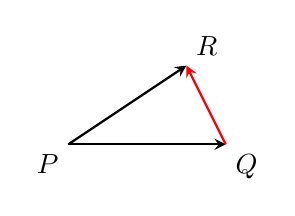
\begin{tikzpicture}
            \coordinate (P) at (0, 0);
            \coordinate (Q) at (2, 0);
            \coordinate (R) at (1.5, 1);
            \draw[thick, -stealth] (P) -- (R);
            \draw[thick, -stealth] (P) -- (Q);
            \draw[red, thick, -stealth] (Q) -- (R);
            \node[above right] at (R) {\(R\)};
            \node[below right] at (Q) {\(Q\)};
            \node[below left] at (P) {\(P\)};
        \end{tikzpicture}
\end{center}
    \item Poiché \(Q \in S_h, \ \vec{PQ} \in V_h\). Allora \(\vec{PR} + \vec{QR} = \vec{PQ} + \vec{v} \in V_h \implies \vec{PR} \in V_h\). Posto \(w = \vec{PR}\), \(t_w(P) = R\) con \(w \in V_h \implies R \in S_h\).
\begin{center}
        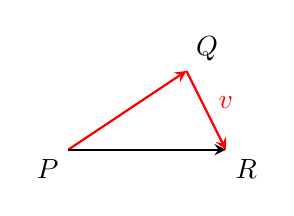
\begin{tikzpicture}
            \coordinate (P) at (0, 0);
            \coordinate (Q) at (2, 0);
            \coordinate (R) at (1.5, 1);
            \draw[red, thick, -stealth] (P) -- (R);
            \draw[thick, -stealth] (P) -- (Q);
            \draw[red, thick, -stealth] (R) -- (Q);
            \node[above right] at (R) {\(Q\)};
            \node[below right] at (Q) {\(R\)};
            \node[below left] at (P) {\(P\)};
            \node[red] at (2, 0.6) {\(v\)};
        \end{tikzpicture}
\end{center}
\end{enumerate}}

\mprop{}{Sia \(S_h=[P, V_h(K)]\) un sottospazio lineare di \(A_n(K)\). Ogni punto di \(S_h\) può essere scelto come origine di \(S_h\). Cioè dato \(Q \in S_h\) abbiamo che \([Q, V_h(K)] = S_h\).}

\pf{Dimostrazione}{Sia \(R \in S_h\). Allora \(\vec{PR} \in V_n\) e \(\vec{PQ}\in V_n\). Quindi \(\vec{QR} = \vec{QP} + \vec{PR} = - \vec{PQ} + \vec{PR} \in V_h \implies \vec{QR} \in V_h\).
\begin{center}
        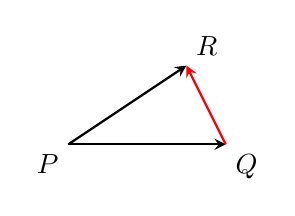
\begin{tikzpicture}
            \coordinate (P) at (0, 0);
            \coordinate (Q) at (2, 0);
            \coordinate (R) at (1.5, 1);
            \draw[thick, -stealth] (P) -- (R);
            \draw[thick, -stealth] (P) -- (Q);
            \draw[red, thick, -stealth] (Q) -- (R);
            \node[above right] at (R) {\(R\)};
            \node[below right] at (Q) {\(Q\)};
            \node[below left] at (P) {\(P\)};
        \end{tikzpicture}
\end{center}
Detto \(w = \vec{QR}\) abbiamo che \(R = t_v(Q)\). \(R\) è traslato di \(Q\) tramite il vettore \(w \in V_h \implies R \in [Q, V_h]\), quindi \[
    S_h \subseteq [Q, V_h]
\] con lo stesso ragionamento scambiamo \(P\) e \(Q\) si dimostra che  \[
[Q, V_h] \subseteq [P, V_h] = S_h
\] e ciò vale solo se \(S_h = [Q, V_h]\).}

\mprop{}{Siano \(S_h\) e \(S_k\) due sottospazi lineari di \(A_n(K)\). Allora \(S_h \subseteq S_k \iff S_h \cap S_k \neq \emptyset\) e \(V_h \le V_k\).}
\pf{Dimostrazione}{"\(\implies \)" Ovviamente \(S_h \cap S_k \neq \emptyset\) e sia \(P \in S_h \cap S_k\). Potremo scrivere \(S_h = [P, V_h]\) e \(S_k = [P, V_k]\). Sia \(v \in V_h\) e sia \(Q = t_v(P) \in S_h \subseteq S_k \implies Q \in S_k\) e sia \(Q = t_v(P)\) ovvero \(\vec{PQ}=v \in V_k \implies V_h \le V_k\).

"\(\impliedby \)" Sia \(P \in S_h \implies [P, V_h] \subseteq [P, V_k]\) (poiché per ipotesi \(V_h \subseteq V_k\)) \([P, V_h] = S_h\) e \([P, V_k]= S_k \implies S_h \subseteq S_k\).}

\mprop{}{Siano \(S_h\) e \(S_k\) sottospazi lineari di \(A_n(K)\). Sia \(S_h \cap S_k \neq \emptyset\) e sia \(P \in S_h \cap S_k\). Allora \[
        S_h \cap S_k = [P, V_h \cap V_k]
\] }

\pf{Dimostrazione}{Sia \(Q \in S_h \cap S_k\). Osserviamo che \(S_h = [P, V_h]\) e \(S_k = [P, V_k]\). \(Q = t_v(P)\) con \(v \in V_h\) (perché \(Q \in S_h\)). Ma \(Q = t_v(P)\) con \(v \in V_k\) (perché \(Q \in S_k\)). Quindi \(Q \in [P, V_h \cap V_k]\) perché \(v \in V_h \cap V_k\), cioè \[
        S_h \cap S_k \subseteq [P, V_h \cap V_k]
\] Viceversa dato \(Q = t_v(P)\) con \(v \in V_h \cap V_k \implies Q \) appartiene sia a \(S_h\) che ad \(S_k\), quindi \(Q \in S_h \cap S_k\), ovvero  \[
[P, V_h \cap V_k] \subseteq S_h \cap S_k
\] \[
\implies [P, V_h \cap V_k] = S_h \cap S_k
\] }

\dfn{Parallelismo tra sottospazi}{Due sottospazi lineari, \(S_p = [P, V_p]\) ed \(S_q = [Q, V_q]\), di \(A_n(K)\) si dicono \textbf{paralleli}, e si scrive \(S_p || S_q\), se i rispettivi spazi di traslazione sono confrontabili, ovvero quando \(V_p \subseteq V_q\), oppure \(V_q \subseteq V_p\).}

\paragraph{Osservazione 1:} La relazione di parallelismo non è transitiva. E' invece riflessiva e simmetrica. Non è quindi una relazione d'equivalenza.
\paragraph{Osservazione 2:} Due sottospazi lineari della stessa dimensione sono paralleli se, e soltanto se, hanno lo stesso spazio di traslazione. Quindi la relazione di parallelismo considerata tra spazi della stessa dimensione è una relazione d'equivalenza.

\mprop{}{Due sottospazi lineari paralleli e di uguale dimensione o coincidono oppure hanno intersezione vuota.}
\dfn{}{
\begin{itemize}
    \item Sia \(S=[P, V_1]\) una retta. Lo spazio \(V_1\) si dice \textbf{direzione} della retta \(S\). Quindi due rette sono parallele se, e soltanto se, hanno la stessa direzione
    \item Sia \(\pi = [P, V_2]\subseteq A_n(K)\) con \(n \ge 2\). Lo spazio \(V_2\) è detto \textbf{giacitura} di \(\pi\). Quindi due piani sono paralleli se, e soltanto se, hanno la stessa giacitura.
    \item Tre o più punti si dicono \textbf{allineati} se esiste una retta che li contiene tutti.
    \item Due o più rette si dicono \textbf{complanari} se esiste un piano che le contiene tutte.
\end{itemize}
}

\section{Proprietà di punti, rette e piani}
\mprop{}{In \(A_n(k)\), con \(n \ge 2\) 
\begin{enumerate}
    \item per ogni due punti distinti passa un'unica retta
    \item per due rette distinte, parallele o incidenti, passa un unico piano
    \item due rette complanari, aventi intersezione vuota, sono parallele
    \item per un punto passa un'unica retta parallela a una retta data (V Postulato di Euclide)
    \item per un punto passa un unico piano, parallelo ad un piano dato
    \item per tre punti, non allineati, passa un unico piano
    \item una retta, avente due punti distinti in un piano, giace nel piano
    \item per un punto passano almeno due rette distinte
\end{enumerate}}

\mprop{}{In \(A_3(K)\),
\begin{enumerate}
    \item una retta e un piano, aventi intersezione vuota, sono paralleli
    \item due piani, aventi intersezione vuota, sono paralleli
    \item due piani distinti, aventi in comune un punto, hanno in comune una retta per quel punto
    \item per una retta passano almeno due piani distinti
\end{enumerate}}

\dfn{Rette sghembe}{In \(A_n(K)\), con \(n \ge 3\), due rette non complanari si dicono \textbf{sghembe}.}
\mprop{}{In \(A_n(K)\), con \(n \ge 3\), esistono due rette \(r_1\) e \(r_2\) sghembe tra loro. Inoltre due rette sghembe \(r_1\) e \(r_2\), sono contenute su due piani \(\pi_1\) e \(\pi_2\) paralleli tra loro e distinti.}

\pf{Dimostrazione}{ Per ipotesi, \(A_n(K)\) ha dimensione almeno 3, quindi esistono nello spazio vettoriale  \(V_n(K)\) almeno 3 vettori linearmente indipendenti. Siano  essi \(u, v, w\). Siano inoltre, \(P\) un punto di \(A\) e \(Q\) il traslato di \(P\) mediante il vettore \(u\) (\(Q = t_u(P)\)). Dimostriamo che le rette \(r = [P, \mcL(v) ]\) ed \(s = [Q, \mcL(w) ]\) sono sghembe. Se infatti, esistesse un piano \(\pi = [P, V_2]\) che le contiene entrambe, lo spazio di traslazione di \(\pi \) conterrebbe 3 vettori linearmente indipendenti, cioè \(v, w\) e \(u = \vec{PQ}\) e ciò è un \textbf{assurdo!}
\begin{figure}[ht]
    \centering
    \def\svgwidth{0.3\columnwidth}
    \incfig{due-rette-complanari-con-3-vettori-linearmente-indipendenti}
    \label{fig:due-rette-complanari-con-3-vettori-linearmente-indipendenti}
\end{figure}
Siano ora \(t = [T, \mcL(v) ]\) e \(t' = [T', \mcL(v') ]\) due rette sghembe. I vettori \(v\) e \(v'\) generano uno spazio vettoriale \(V_2\) di dimensione 2. Pertanto, i piani  \(\pi = [T, V_2]\) e \(\pi' = [T', V_2]\), che risultano paralleli, sono distinti e contengono, rispettivamente le rette \(t\) e \(t'\).}

\section{Geometria analitica in \(A_n(\RR )\)}
\dfn{Riferimento affine}{Si dice \textbf{riferimento affine} di \(A_n(\RR )\) una coppia \(RA = [O,B]\) costituita da un punto \(O\) fissato, detto origine, e da una base \(B\) dello spazio vettoriale \(V_n(\RR )\).}

\dfn{Coordinate}{Fissato, in \(A_n(\RR )\), un riferimento affine \(RA = [O,B]\), si dicono \textbf{coordinate} del punto \(P\) in \(RA\) le componenti, in \(B\), del vettore \(\vec{OP}\) e si scrive \(P=(x_i)_{i \in I_n}\).}

\begin{enumerate}
\item In \(A_1(\RR )\), un riferimento affine è una coppia \(RA = [O,B]\), ove \(O\) è un punto fissato e \(B = (e_1)\) è una base di \(V_1(\RR )\). Se \(\vec{OP}=xe_1\), si scrive \(P=(x)\) e si dice che \(x\) è l'\textbf{ascissa} del punto \(P\) in \(RA\). 
\begin{figure}[ht]
    \centering
    \def\svgwidth{0.5\columnwidth}
    \incfig{ascissa}
    \label{fig:ascissa}
\end{figure}
\item In \(A_2(\RR )\), un riferimento affine è una coppia \(RA = [O,B]\), ove \(O\) è un punto fissato e \(B = (e_1, e_2)\) è una base di \(V_2(\RR )\). La retta \([O, \mcL(e_1) ]\) è detta \textbf{asse delle ascisse} e la retta \([O, \mcL(e_2) ]\) è detta \textbf{asse delle ordinate}. Se \(\vec{OP} = xe_1 + y e_2\), si scrive \(P = (x, y)\) e si dice che \((x,y)\) è la coppia delle coordinate di \(P\) in \(RA\), dette rispettivamente \textbf{ascissa} e \textbf{ordinata} del punto \(P\).
\begin{figure}[ht]
    \centering
    \def\svgwidth{100pt}
    \incfig{ascissa-e-ordinata}
    \label{fig:ascissa-e-ordinata}
\end{figure}
\item In \(A_3(\RR )\), un riferimento affine è una coppia \(RA = [O,B]\), ove \(O\) è un punto fissato e \(B = (e_1, e_2, e_3)\) è una base di \(V_3(\RR )\). La retta \([O, \mcL(e_1) ]\) è detta \textbf{asse delle ascisse}, la retta \([O, \mcL(e_2) ]\) è detta \textbf{asse delle ordinate} e la retta \([O, \mcL(e_3) ]\) è detta \textbf{asse delle quote}. Sono detti \textbf{piani coordinati} i piani \(xy = [O, \mcL(e_1, e_2) ], xz = [O, \mcL(e_1, e_3) ]\) e \(yz = [O, \mcL(e_2, e_3) ]\). Inoltre, se \(\vec{OP}=xe_1+ ye_2 + ze_3\), si scrive \(P = (x, y,z)\) e si dice che \((x, y, z)\) è la terna delle coordinate di \(P\) in \(RA\), dette rispettivamente \textbf{ascissa, ordinata} e \textbf{quota} del punto \(P\).
\begin{figure}[ht]
    \centering
    \def\svgwidth{200pt}
    \incfig{terne-di-coordinate}
    \label{fig:terne-di-coordinate}
\end{figure}
\end{enumerate}

\thm{}{In \(A_n(K)\), con \(RA = [O, B]\), siano \(P = (x_1', x_2', \ldots , x_n')\) e \(Q = (x_1 '', x_2 '', \ldots  , x_n '')\) due punti di \(A\). Allora le componenti di \(\vec{PQ}\) rispetto a \(B\) sono \[
(x_1 '' - x_1', x_2 '' - x_2' , \ldots, x_n '' - x_n')
\] }

\pf{Dimostrazione}{Posti due vettori \[
\vec{OP} : \ x_1' e_1+ x_2' e_2 + \ldots + x_n' e_n
\] \[
\vec{OQ}: \ x_1 '' e_1 + x_2 '' e_2 + \ldots + x_n '' e_n
\]Per la proprietà della definizione di spazio affine possiamo dire che \[
\vec{PQ} = \vec{PO} + \vec{OQ} = \vec{OQ} - \vec{OP} = \sum_{i \in I_n} (x_i '' - x_i') e_i
\] }
Posti \[
 X '' = \left( \; \begin{matrix} x ''_1 \\ x ''_2\\ \vdots \\ x ''_n \end{matrix} \; \right), X' = \left( \; \begin{matrix} x'_1 \\ x'_2\\ \vdots \\ x'_n \end{matrix} \; \right) \text{ e } T = \left( \; \begin{matrix} t_1 \\ t_2\\ \vdots \\ t_n \end{matrix} \; \right)
\] si ottiene l'equivalente, ma spesso più agevole, forma matriciale: \[
X '' - X' = T
\] che può essere riscritta come \[
X '' = X' + T
\] Da quest'ultima equazione si vede che le coordinate del traslato del punto \(P = (x_1', x_2', \ldots , x_n')\), attraverso il vettore \(v\) di componenti \((t_1, t_2, \ldots , t_n)\), si ottengono sommando, ordinatamente, alle coordinate di \(P\) le componenti del vettore di traslazione. Per questo le relazioni che compaiono nell'equazione sono anche dette \textbf{equazioni della traslazione individuata da \(v\)}.

\dfn{Punto medio}{Dato \(P\) e \(Q \in A\) (insieme dei punti di \(A_n(\RR )\)), definiamo il punto medio del segmento \([PQ]\) come \[
M = t_{1/2 \vec{PQ}} (P)
\] 
\begin{center}
    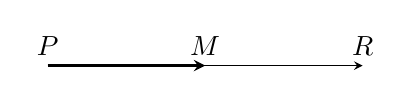
\begin{tikzpicture}
        \coordinate (P) at (0, 0);
        \coordinate (M) at (2, 0);
        \coordinate (R) at (4, 0);
        \draw[thick, -stealth] (P) -- (M);
        \draw[thin, -stealth] (P) -- (R);
        \node[above] at (R) {\(R\)};
        \node[above] at (M) {\(M\)};
        \node[above] at (P) {\(P\)};
    \end{tikzpicture}
\end{center}}

\mprop{}{Dati \(P, Q \in A\) e dato un riferimento affine \(RA = [O, B]\) abbiamo che le coordinate del punto medio di \(P\) e \(Q\) sono le semisomme delle coordinate omonime di \(P\) e di \(Q\).}

\dfn{Punto simmetrico}{In \(A_n(\RR )\) dati i punti \(P\) e \(C\) diremo che \(S\) è il \textbf{punto simmetrico} di \(P\) rispetto a \(C\) se \(C\) è il punto medio di \([P, S]\).}

\section{Rappresentazioni analitiche}
\dfn{Equazioni parametriche di una retta in \(A_n(\RR )\)}{Sia \(RA = [O,B]\) un riferimento fissato in \(A_n(\RR )\), ove \(B = (e_1, e_2, \ldots , e_n)\). Sia \(r = [P, V_1 = \mcL(v) ]\) la retta di origine il punto \(P = (x_1', x_2', \ldots , x_n')\) e spazio di traslazione generato da \(v = (l_1, l_2, \ldots , l_n)\). Il generico vettore \(w\) di \(\mcL(v) \) è proporzionale al vettore \(v\), cioè \(w = tv\), con \(t \in \RR \), quindi, \(w = (tl_1, tl_2, \ldots , tl_n)\). Dato che la retta \(r\) è il luogo dei traslati di \(P\) attraverso i vettori di \(\mcL(v) \), applicando le equazioni del teorema precedente si ottengono le coordinate del generico punto di \(r\) \[
\begin{cases}
    \ x_1 = x_1' + l_1t \\
    \ x_2 = x_2' + l_2t \\
    \ \ldots \ldots \ldots \ldots \\
    \ x_n = x_n' + l_nt \\
\end{cases} \quad \text{con} \quad t \in \RR , \quad (l_1, l_2, \ldots , l_n) \neq \ul{0} 
\] tali equazioni sono dette \textbf{equazioni parametriche} di \(r\) in \(A_n(\RR )\). Al variare di \(t \in \RR \), si ottengono le coordinate di tutti i punti di una retta e, quindi, tutti i punti di una retta sono \(\infty^{1}\).}

\dfn{Parametri direttori}{Si dicono \textbf{parametri direttori} di \(r = [P, V_1]\), le componenti di un qualunque vettore nullo di \(V_1\).}
\paragraph{Osservazione:} I parametri direttori di una retta sono, quindi, determinati a meno di un fattore non nullo di proporzionalità. Definiamo la classe dei parametri direttori di \(r\) come \(p.d.r = [(l_1, l_2, \ldots , l_n)]\) con \((l_1, l_2, \ldots , l_n)\) un qualsiasi vettore appartenente a \(V_1\).

\subsubsection{Equazioni parametriche di una retta in \(A_2(\RR )\)} 
In \(A_2(\RR )\), sia fissato un riferimento \(RA = [O, B]\), ove \(B = (e_1, e_2)\). Una retta \(r = [P, V_1]\) è il luogo dei traslati di un punto \(P\) mediante i vettori di \(V_1 \subset V_2\). Se \(P\) ha coordinate \((x_0, y_0)\) e \(V_1 = \mcL(v) \), ove \(v = le_1 + me_2\), le equazioni della definizione diventano \[
\begin{cases}
    \ x = x_0 + lt \\
    \ y = y_0 + mt \\
\end{cases}
\quad \text{ove}\quad t \in \RR , \quad (l,m) \neq (0,0)\] 
e sono dette \textbf{equazioni parametriche} di \(r\) in \(A_2(\RR )\).

\subsubsection{Equazioni parametriche di una retta in \(A_3(\RR )\)}
In \(A_3(\RR )\), sia fissato un riferimento \(RA = [O, B]\), ove \(B = (e_1, e_2, e_3)\). Una retta \(r = [P, V_1]\) è il luogo dei traslati di un punto \(P\) mediante i vettori di \(V_1 \subset V_3\). Se \(P\) ha coordinate \((x_0, y_0, z_0)\) e \(V_1 = \mcL(v) \), ove \(v = le_1 + me_2 + ne_3\), le equazioni della definizione diventano \[
\begin{cases}
    \ x = x_0 + lt \\
    \ y = y_0 + mt \\
    \ z = z_0 + nt \\
\end{cases}
\quad \text{ove}\quad t \in \RR , \quad (l,m,n) \neq (0,0,0)\] 
e sono dette \textbf{equazioni parametriche} di \(r\) in \(A_3(\RR )\).

\paragraph{Osservazione:} In modo del tutto analogo possiamo determinare le equazioni parametriche di sottospazi lineari di dimensione \(n\), che quindi dipenderanno da \(n\) parametri.

\subsubsection{Equazione cartesiana di una retta in \(A_2(\RR )\)}
In \(A_2(\RR )\) una retta si può rappresentare attraverso le sue equazioni parametriche in questo modo \[
\begin{cases}
    \ x = x_p + lt \\
    \ y = y_p + mt \\
\end{cases}
\] possiamo convertire questo sistema lineare in forma matriciale e quindi \[
\left( \;
\begin{matrix}
    x \\
    y \\
\end{matrix} \;
\right) = 
\left( \; \begin{matrix}
    x_p \\
    y_p \\
\end{matrix} \; \right) +
t  
\left( \; \begin{matrix}
    l \\
    m \\
\end{matrix} \; \right) \iff 
\left( \; \begin{matrix}
    x - x_p \\
    y - y_p \\
\end{matrix} \; \right) = t
\left( \; \begin{matrix}
    l \\
    m \\
\end{matrix} \; \right) \iff 
\left| \;
\begin{matrix}
    x - x_p & y - y_p \\
    l & m \\
\end{matrix} \;
\right| = 0
\] 
Quindi vale la relazione \[
    ((x-x_p) m) (l (y-y_p)) = mx - ly -mx_p + ly_p = 0
\] Possiamo raggruppare i termini noti \(-mx_p + ly_p\) in un generico termine \(c\) e quindi l'equazione cartesiana della retta diventa \[
ax + by + c = 0 \quad \text{con}\quad (a,b) \neq (0,0)
\] Quindi i parametri direttori della generica retta \(r\) saranno \(p.d.r = [(l,m)] = [(-b, a)]\).

\subsubsection{Mutua posizione di due rette in \(A_2(\RR )\)}
Siano due rette \[
r: ax + by + c = 0 \quad (a,b) \neq (0,0)
\] \[
s: a'x + b'y + c' = 0 \quad (a', b') \neq (0,0)
\]
La loro intersezione può essere \[ r \cap s = \
\begin{cases}
    \ \text{un unico punto se \(r\) e \(s\) sono incidenti} \\
    \ \emptyset \text{ se \(r\) e \(s\) sono parallele e distinte} \\
    \ r \equiv s \text{ se sono coincidenti } \\
\end{cases}
\]
Consideriamo il sistema \[r \cap s=
\begin{cases}
    \ ax + by + c = 0 \\
    \ a'x + b'y + c' = 0 \\
\end{cases}
\]
Le coordinate dei punti di \(r \cap s\) sono le soluzioni del sistema. Posti \[
A =
\left( \; \\
 \begin{matrix}
    a & b \\
    a' & b' \\
\end{matrix} \; \\
 \right) \quad \text{la matrice incompleta del sistema,}
 \quad A|B =
\left( \; \\
 \begin{matrix}
    a & b & -c \\
    a' & b' & -c' \\
\end{matrix} \; \\
 \right) \quad \text{la matrice completa del sistema}
\] possiamo dire che \(\rho(A) \ge 1\) poiché abbiamo richiesto che \((a,b) \neq (0,0)\) e \(\rho(A) \le 2\). Quindi abbiamo due casi possibili
\begin{enumerate}
    \item se \(\rho(A) = 2 \implies \rho(A) = \rho(A|B) =2\), quindi il sistema è compatibile e ha \(\infty^{2-2}\) soluzioni \(\implies \exists !\) soluzione del sistema \(\implies r \cap s = \{P\} \implies r \cap s\) sono \textbf{incidenti}.
    \item se \(\rho(A) = 1\) allora \(r || s\), ma non sappiamo se esse siano parallele e distinte o se esse coincidano. Perciò dobbiamo suddividere in due sottocasi
        \begin{enumerate}
            \item se fossero parallele e distinte il sistema non sarebbe compatibile, perciò \(2= \rho(A|B) > \rho(A) = 1\)
            \item se invece \(\rho(A) = 1\) e \(\rho(B) = 1\) il sistema ammette \(\infty^{2-1}\) soluzioni, perciò \(r \equiv s \implies r||s\) se \(\rho(A) = 1\)
        \end{enumerate}
\end{enumerate}
\subsubsection{Fasci di rette in \(A_2(\RR )\)}
\dfn{Fascio improprio di rette}{Si dice \textbf{fascio improprio di rette} l'insieme di tutte e sole le rette del piano \(A_2(\RR )\) parallele ad una retta data.}
\mprop{}{Una retta appartiene al fascio improprio di rette parallele alla retta \(r = [P, V_1]: ax + by + c = 0, \ (a,b) \neq (0,0)\), se, e soltanto se, ha un'equazione del tipo \[
ax + by + k = 0 \quad \text{ove} \quad k \in \RR 
\] detta \textbf{equazione del fascio improprio di rette}. Da cui si deduce che le rette di un fascio improprio di rette sono \(\infty^{1}\)}
\paragraph{Osservazione:} Tutte e sole le rette parallele ad \(r\) hanno parametri direttori \([(-b, a)]\) e quindi \(r\) e \(s\) sono la stessa retta \(\iff (a,b,c) \sim (a',b', c')\).

\dfn{Fascio proprio di rette}{Si dice \textbf{fascio proprio di rette} l'insieme di tutte le rette di \(A_2(\RR )\) passanti per un punto \(P\) dato, detto \textbf{centro} o \textbf{sostegno} del fascio.}

\mprop{}{Siano \(r: ax + by + c = 0\) e \(r': a'x + b'y + c' = 0\), con \((a,b) \neq (0,0)\) e \((a', b') \neq (0,0)\), due distinte rette incidenti in un punto \(P\). Una retta \(s\) appartiene al fascio di centro \(P\) se, e soltanto se, ha un'equazione di tipo \[
\lambda (ax + by + c) + \mu(a'x+ b'y + c') = 0 \quad \text{ove} \quad \lambda , \mu \in \RR \quad e \quad (\lambda , \mu) \neq (0,0)
\] detta \textbf{equazione del fascio proprio di rette}. Se nell'equazione risulta \(\lambda  \neq 0\), posto \(k = \mu / \lambda \), si ottiene \[
ax + by + c + k (a'x + b'y + c') = 0 \quad \text{ove} \quad k \in \RR 
\] detta \textbf{equazione ridotta del fascio proprio di rette}, in cui, ovviamente, la retta \(r' : a'x + b'y + c' = 0\) non è rappresentata. Quindi possiamo dire che le rette di un fascio proprio di rette sono \(\infty^{1}\).}

\subsubsection{Simmetrie in \(A_2(\RR )\)}
\dfn{Simmetria rispetto ad una retta}{Il punto \(T\) si dice \textbf{simmetrico} del punto \(H\), rispetto alla retta \(r = [P, V_1]\), detta \textbf{asse di simmetria}, nella direzione \(W_1 \neq V_1\), se lo è nella simmetria di centro \(C = r \cap s\), dove \(s = [H, W_1]\). Tale simmetria si dice anche \textbf{simmetria rispetto ad una retta in una direzione assegnata}.}

\begin{figure}[ht]
    \centering
    \def\svgwidth{160pt}
    \incfig{simmetria-punto-retta}
    \label{fig:simmetria-punto-retta}
\end{figure}

\subsubsection{Equazione cartesiana di un piano in \(A_3(\RR )\)}
In \(A_3(\RR )\) dato il \(RA = [O, B]\), con \(B = (e_1, e_2, e_3)\). Sia \(\alpha = [P, V_2]\) un piano con \(P = (x_p, y_p, z_p)\) e \(V_2 = \mcL(v, v') \) (con \(v \neq kv'\)), tali che  \[
v = le_1 + me_2 + ne_3 \qquad 
v' = l'e_1 + m'e_2 + n'e_3
\] 
Il generico vettore \(w \in V_2\) si scrive come \(w = tv + t' v'\). Quindi \(t_w(P)\) è il generico punto appartenente a \(\alpha \). Di conseguenza possiamo dire che \[
\begin{cases}
    \ x = x_p + tl + t'l' \\
    \ y = y_p + tm + t'm' \\
    \ z = z_p + tn + t'n' \\
\end{cases} \implies 
\left( \;
 \begin{matrix}
    x \\
    y \\
    z \\
\end{matrix} \;
 \right) =
\left( \;
 \begin{matrix}
    x_p \\
    y_p \\
    z_p \\
\end{matrix} \;
 \right) +
\left( \;
 \begin{matrix}
    tl + t'l' \\
    tm + t'm' \\
    tn + t'm' \\
\end{matrix} \;
 \right) 
\] cioè, per l'equazione della traslazione \(\left( \; \begin{matrix} x \\ y\\ z \end{matrix} \; \right) \) sono le coordinate del generico punto di \(\alpha \). Date dalla somma di \(\left( \; \begin{matrix} x_p \\ y_p\\ z_p \end{matrix} \; \right) \) cioè le coordinate di \(P\) con \(\left( \; \begin{matrix} tl + t'l' \\ tm + t'm'\\ tn + t'n' \end{matrix} \; \right) \) cioè le componenti di \(w\).

Seguendo un ragionamento analogo a quello fatto per le rette in \(A_2(\RR )\) possiamo descrivere un piano in \(A_3(\RR )\) come \[
\left| \; \begin{matrix}
    x-x_p & y-y_p & z-z_p \\
    l & m & n \\
    l' & m' & n' \\
\end{matrix} \; \right| = 0
\] e da questa ne ricaviamo la seguente equazione \[
ax + by + cz + d = 0 \quad \text{con} \quad  (a,b,c) \neq (0,0,0)
\] detta \textbf{equazione cartesiana} del piano in \(A_3(\RR )\). Tale equazione è definita a meno di un fattore di proporzionalità non nullo.

\subsubsection{Equazioni cartesiane delle rette in \(A_3(\RR )\)}

Fissiamo un \(RA = [O, B]\) con \(B = (e_1, e_2, e_3)\) e data una retta \(r = [P, V_1=\mcL(l,m,n) ]\) possiamo scrivere l'equazione parametrica della retta \[
r : \
\begin{cases}
    \ x = x_p + tl \\
    \ y = y_p + tm \\
    \ z = z_p + tn \\
\end{cases} \quad \text{con}\quad (l,m,n) \neq (0,0,0)
\] Da cui deriva la seguente relazione \[
\frac{x-x_p}{l} = \frac{y-y_p}{m} = \frac{z - z_p}{n}
\] in particolare, se poniamo ad esempio \(l \neq 0\), otteniamo il seguente sistema \[
\begin{cases}
    \ y = \frac{m}{l} (x-x_p) + y_p \\
    \ z = \frac{n}{l} (x-x_p) + z_p \\
\end{cases} \implies 
\begin{cases}
    \ y = \frac{m}{l} x + k \\
    \ z = \frac{n}{l} x + h \\
\end{cases} \ \text{ove} \quad h, k \in \RR 
\] esistono, ovviamente le equazioni relative ai casi \(m \neq 0\) e \(n \neq 0\) e, dato che la terna \((l,m,n)\) è non nulla, ogni retta ammette sempre, almeno, una rappresentazione simile. In ogni caso, qualunque essa sia, possiamo concludere che una retta si rappresenta con un sistema di due equazioni lineari nelle incognite \(x, y\) e \(z\), in cui il rango della matrice incompleta è uguale a 2. E infatti sussiste anche il viceversa, cioè \[
\begin{cases}
    \ ax + by + cz + d = 0 \\
    \ a'x + b'y + c'z + d' = 0 \\
\end{cases} \ \text{con} \quad \rho
\left( \; \begin{matrix}
    a & b & c \\
    a' & b' & c' \\
\end{matrix} \; \right) = 2
\] rappresenta una retta. Infatti per il teorema di Rouché-Capelli il sistema è compatibile e ammette \(\infty^{1}\) soluzioni, cioè le sue soluzioni dipendono da un solo parametro.  

Analogamente a quanto già osservato in \(A_2(\RR )\), dalla precedente equazione deriva che le componenti, dei vettori dello spazio di traslazione della retta \(r\), sono le soluzioni del sistema omogeneo associato a una rappresentazione cartesiana di \(r\) stessa. Quindi possiamo dedurre la classe dei parametri direttori della retta \(r\) attraverso la regola dei minori. L'insieme delle \(\infty^{1}\) soluzioni del sistema omogeneo \[
\begin{cases}
    \ ax + by + cz + d = 0 \\
    \ a'x + b'y + c'z + d' = 0 \\
\end{cases} \ \text{con} \quad \rho
\left( \; \begin{matrix}
    a & b & c \\
    a' & b' & c' \\
\end{matrix} \; \right) = 2
\] è \[
\left\{ \left( t
\left| \; \begin{matrix}
    b & c \\
    b' & c' \\
\end{matrix} \; \right|,
-t
\left| \; \begin{matrix}
    a & c \\
    a' & c' \\
\end{matrix} \; \right|, t
\left| \; \begin{matrix}
    a & b \\
    a' & b' \\
\end{matrix} \; \right| \right)
: \ t \in R \right\}
\] 
\subsubsection{Mutua posizione di due piani in \(A_3(\RR )\)}
Fissato un \(RA\) e dati due piani in \(A_3(\RR )\)\[
\alpha : ax + by + cz + d = 0 \qquad \alpha' : a'x + b'y + c'z + d' = 0
\] la loro intersezione è data dal sistema \[
\alpha \cap \alpha' : \
\begin{cases}
    \ ax + by + cz + d = 0 \\
    \ a'x + b'y + c'z + d' = 0 \\
\end{cases}
\] Quindi possiamo distinguere in 3 casi:
\begin{enumerate}
    \item \(\rho(A) = 2 \implies \rho(A) = \rho(A|B) = 2 \) quindi il sistema è compatibile e ammette \(\infty^{3-2} = \infty^{1}\) soluzioni \(\implies \alpha \cap \alpha' = r\), quindi \(\alpha \) e \(\alpha'\) sono due piani \textbf{incidenti}.
    \item Nel caso in cui \(\rho(A) = 1\) dobbiamo distinguere in due sottocasi
        \begin{enumerate}
            \item \(\rho(A|B) = 2 \) e \(\rho(A) = 1\), il sistema non è compatibile, quindi \(\alpha \cap \alpha' = \emptyset\) e \(\alpha \) è parallelo e distinto da \(\alpha'\). \(\alpha \) e \(\alpha'\) sono detti \textbf{paralleli e distinti}.
            \item \(\rho(A) = 1\) e \(\rho(A|B) = 1\), il sistema è compatibile e ammette \(\infty^{3-1} = \infty^{2}\) soluzioni. Quindi l'insieme delle soluzioni dipende da due parametri \(\implies \alpha \equiv \alpha'\).
        \end{enumerate}
\end{enumerate}

\mprop{Condizione di parallelismo tra piani}{\(\alpha || \alpha' \iff \rho(A) = 1 \iff a = ka' \ b = kb' \ c = kc' \iff [(a,b,c)] = [(ka',kb',kc')] = [(a', b', c')]\). Questa viene denominata condizione analitica di parallelismo tra piani.}

\subsubsection{Fasci di piani in \(A_3(\RR )\)}
\dfn{Fascio improprio di piani}{Si dice \textbf{fascio improprio di piani} l'insieme di tutti e soli i piani di \(A_3(\RR )\) paralleli a un piano dato.}
\mprop{}{Un piano appartiene al fascio improprio di piani paralleli ad \(\alpha =[P, V_2]: ax + by + cz + d = 0\), con \((a,b,c) \neq (0,0,0)\), se, e soltanto se, ha un'equazione del tipo \[
ax + by + cz + k = 0 \quad \text{ove} \quad k \in \RR 
\] detta \textbf{equazione del fascio improprio di piani}. I piani di un fascio improprio sono \(\infty^{1}\).}

\dfn{Fascio proprio di piani}{Si dice \textbf{fascio proprio di piani}, l'insieme di tutti e soli i piani di \(A_3(\RR )\) passanti per una retta data \(r\), detta \textbf{asse} o \textbf{sostegno} del fascio.}
\mprop{}{Siano \(r\) una retta, \(\alpha : ax + by + cz + d = 0\) e \(\alpha' : a'x + b'y + c'z + d' = 0\), con \((a,b,c) \neq (0,0,0)\) e \((a',b',c') \neq (0,0,0)\), due distinti piani per \(r\). Un piano \(\beta \) appartiene al fascio di sostegno \(r\) se, e soltanto se, ha un'equazione del tipo \[
\lambda (ax+by+cz+d) + \mu (a'x + b'y +c'z+d') = 0 \quad \text{ove}\quad \lambda , \mu \in \RR \quad e \quad (\lambda , \mu) \neq (0,0)
\] detta \textbf{equazione del fascio proprio di piani}. Se nell'equazione risulta \(\lambda \neq 0\), posto \(h = \mu / \lambda \), si ottiene \[
ax + by + cz + d + h(a'x + b'y + c'z + d') = 0 \quad \text{ove} \quad h \in \RR 
\] detta \textbf{equazione ridotta del fascio proprio di piani}, in cui ovviamente il piano \(\beta : a'x + b'y + c'z + d' = 0\) non è rappresentato. Dalla rappresentazione ridotta del fascio si deduce che i piani di un fascio proprio sono \(\infty^{1}\).}

\subsubsection{Mutua posizione di due rette in \(A_3(\RR )\)}
Siano assegnate le rette \[
r :
\begin{cases}
    \ ax + by + cz + d = 0 \\
    \ a'x + b'y + c'z + d' = 0 \\
\end{cases} \quad \rho
\left( \; \begin{matrix}
    a & b & c \\
    a' & b' & c' \\
\end{matrix} \; \right) = 2
\] \[
s :
\begin{cases}
    \ a ''x + b ''y + c ''z + d '' = 0 \\
    \ a'''x + b'''y + c'''z + d''' = 0 \\
\end{cases} \quad \rho
\left( \; \begin{matrix}
    a ''& b '' & c ''\\
    a''' & b''' & c''' \\
\end{matrix} \; \right) = 2
\] Sia \[
r \cap s:
\begin{cases}
    \ ax + by + cz + d = 0 \\
    \ a'x + b'y + c'z + d' = 0 \\
    \ a ''x + b ''y + c ''z + d '' = 0 \\
    \ a'''x + b'''y + c'''z + d''' = 0 \\
\end{cases}
\] il sistema costituito dalle loro equazioni e siano \(A\) e \(A|B\) le matrici incompleta e completa associate al sistema. \[
AX = B \quad \text{con} \quad B =
\left( \; \begin{matrix}
    -d \\
    -d' \\
    -d'' \\
    -d''' \\
\end{matrix} \; \right) 
\quad X = 
\left( \; \begin{matrix}
    x \\
    y \\
    z \\
\end{matrix} \; \right) 
\quad A =
\left( \; \begin{matrix}
    a & b & c \\
    a' & b' & c' \\
    a '' & b '' & c '' \\
    a''' & b''' & c''' \\
\end{matrix} \; \right) 
\] Esaminiamo i 4 casi possibili:

\begin{enumerate}
    \item \(\rho(A|B) = 4 \implies \rho(A) = 3\) poiché \(A|B\) è ottenuta aggiungendo una colonna ad \(A\), quindi \(\rho(A|B) \le \rho(A) + 1 \implies \rho(A) =3 \). Il sistema non è compatibile per il teorema di Rouché-Capelli \(\implies r  \) e \(s\) sono o parallele e disgiunte, oppure sghembe. Ma siccome \(\rho(A) = 3 \implies r = [P,V_1] \quad s =[P', V_1'] \quad V_1 \neq V_1' \implies r\) non è parallela ad \(s\). Quindi \(r\) e \(s\) sono \textbf{sghembe}.
    \item \(\rho(A|B) = 3\) e \(\rho(A) =3\). Il sistema è compatibile e per il teorema di Rouché-Capelli  esiste un'unica soluzione \(r \cap s = \{P\} \implies r\) e \(s\) si dicono \textbf{incidenti}.
    \item \(\rho(A|B) = 3\) e \(\rho(A) = 2\). Il sistema non è compatibile per il teorema di R.C. Siccome \(\rho(A) =2 \implies V_1= V_1' \implies r\) è parallela a \(s\) e \(r \neq s\). Si dice che \(r\) e \(s\) sono \textbf{parallele e distinte}.
    \item \(\rho(A|B) = \rho(A) = 2\) il sistema è compatibile e ammette \(\infty^{1}\) soluzioni. Si dice che  le rette \(r\) e \(s\) sono \textbf{coincidenti}.
\end{enumerate}

\dfn{Stella propria di rette}{In \(A_3(\RR )\) si dice \textbf{stella propria} di rette, l'insieme di tutte e sole le rette passanti per un ponto assegnato.}
\paragraph{Osservazione:} Possiamo scrivere la rappresentazione di tutte e sole le rette della stella passanti per \(P = (x_0, y_0, z_0)\) come \[
\alpha :
\begin{cases}
    \ x = x_0 + tl \\
    \ y = y_0 + tm \\
    \ z = z_0 + tn \\
\end{cases}
\] e da qui abbiamo che \[
t = \frac{x-x_0}{l}= \frac{y-y_0}{m} = \frac{z-z_0}{n} = 
\begin{cases}
    \ m(x-x_0) = l(y-y_0) \\
    \ n (x-x_0) = l(z-z_0) \\
\end{cases}
\] dividendo per \(l\) (supponendo \(l \neq 0\)) si ottiene che abbiamo solo due parametri liberi e quindi abbiamo \(\infty^{2}\) rette nella stella di rette per \(P\).

\dfn{Stella impropria di rette}{In \(A_3(\RR )\) si dice \textbf{stella impropria} di rette, l'insieme di tutte e sole le rette parallele ad una retta data.}

\paragraph{Osservazione:} Una rappresentazione analitica di tutte le rette parallele a una retta assegnata, di parametri direttori \((l,m,n)\), è \[
\beta : 
\begin{cases}
    \ x = x' + tl \\
    \ y = y' + tm \\
    \ z = z' + tn \\
\end{cases} \iff  
\begin{cases}
    \ m(x-x') = l(y-y') \\
    \ n(x-x') = l(z-z') \\
\end{cases}
\] Questa volta non sono i parametri direttori ad essere i parametri, ma i punti di \(P = (x', y', z')\). Quest'ultima è detta \textbf{equazione cartesiana della stella impropria} di \(r\). Abbiamo \(\infty^2\) rette in \(A_3(\RR )\) parallele ad una retta data.

\subsubsection{Mutua posizione di due piani in \(A_3(\RR )\)}
Siano \[
\alpha = [P, V_2]: ax + by + cz + d = 0, \quad \text{con}\quad (a,b,c) \neq (0,0,0) \]
\[
r=[Q, V_1]:
\begin{cases}
    \ a'x + b'y + c'z + d' = 0 \\
    \ a ''x + b ''y + c ''z + d '' = 0 \\
\end{cases} \text{con} \quad 
\rho
\left( \; \begin{matrix}
    a' & b' & c' \\
    a '' & b '' & c '' \\
\end{matrix} \; \right) = 2
\] e sia \(r \cap \alpha \) rappresentato dal sistema lineare \(AX = B\), dove \[
A =
\left( \; \begin{matrix}
    a & b & c \\
    a' & b' & c' \\
    a '' & b '' & c '' \\
\end{matrix} \; \right) \quad
B =
\left( \; \begin{matrix}
    -d \\
    -d' \\
    -d '' \\
\end{matrix} \; \right) \quad X =
\left( \; \begin{matrix}
    x \\
    y \\
    z \\
\end{matrix} \; \right) 
\] Sono 3 i casi possibili
\begin{enumerate}
    \item sia \(\rho(A|B) = \rho(A) =3\), il sistema è compatibile e, per il teorema di R.C. ammette un'unica soluzione \(r \cap \alpha  = \{P\} \implies r\) e \(\alpha \) si dicono \textbf{incidenti}
    \item \(\rho(A|B) = 3\) e \(\rho(A) =2\), il sistema non è compatibile, quindi \(r || \alpha \) e \(r \notin \alpha \) 
    \item \(\rho(A|B) = 2\) e \(\rho(A) = 2\), il sistema è compatibile e ammette \(\infty^{1}\) soluzioni, quindi \(r\) è contenuto in \(\alpha \)(\(r\) è anche chiaramente parallelo ad \(\alpha \))
\end{enumerate}

\paragraph{Osservazione:} \(\rho(A) = 2 \iff r || \alpha \) ovvero \[
\left| \; \begin{matrix}
    a & b & c \\
    a' & b' & c' \\
    a '' & b '' & c '' \\
\end{matrix} \; \right| = 0 \iff 
a \underbrace{
\left| \; \begin{matrix}
    b' & c' \\
    b '' & c '' \\
\end{matrix} \; \right|
}_{ \Gamma_1 \to l } 
- b 
\underbrace{
\left| \; \begin{matrix}
    a' & b' \\
    a '' & c '' \\
\end{matrix} \; \right| 
}_{\Gamma_2 \to m} 
+ c
\underbrace{
\left| \; \begin{matrix}
    a' & b' \\
    a '' & b '' \\
\end{matrix} \; \right|
}_{\Gamma_3 \to n} = 0
\] Quindi posti i parametri direttori \([(l,m,n)]\) possiamo dare la
\mprop{Condizione di parallelismo tra retta e piano}{La condizione di parallelismo tra retta e piano si esprime come \[
al + bm + cn = 0
\] dove \([(l,m,n)]\) sono i parametri direttori della retta e il piano è \(ax + by + cz + d = 0\).}

\dfn{Stella impropria di piani}{Si dice \textbf{stella impropria di piani} l'insieme di tutti e soli i piani di \(A_3(\RR )\) paralleli ad una retta data.}
\paragraph{Osservazione:} Chiaramente dalla proposizione precedente segue che dati parametri direttori \([(l,m,n)]\) abbiamo che esistono \(\infty^{2}\) piani appartenenti alla stella impropria di piani.

\dfn{Stella propria di piani}{Si dice \textbf{stella propria di piani} l'insieme di tutti e soli i piani di \(A_3(\RR )\) passanti per un punto  assegnato detto \textbf{centro} o \textbf{sostegno} della stella.}
\paragraph{Osservazione:} Analogamente abbiamo \(\infty^{2}\) piani nella stella propria di piani.

\subsubsection{Simmetrie in \(A_3(\RR )\)}
\dfn{Simmetrico rispetto a una retta e una giacitura assegnata}{Il punto \(T\) si dice \textbf{simmetrico} del punto \(H\), rispetto alla retta \(r=[Q, V_1]\), nella giacitura \(V_2 \not\supseteq V_1\), se è simmetrico di \(H\) rispetto al punto \(C = \alpha  \cap r\), dove \(\alpha = [H, V_2]\).}

\begin{figure}[ht]
    \centering
    \def\svgwidth{150pt}
    \incfig{simmetria-retta-giacitura}
    \label{fig:simmetria-retta-giacitura}
\end{figure}

\dfn{Simmetria rispetto a un piano in una direzione assegnata}{Un punto \(T\) si dice \textbf{simmetrico} del punto \(H\), rispetto al piano\(\alpha = [Q, V_2]\), nella direzione \(V_1 \not\supseteq V_2\), se è simmetrico di \(H\) rispetto al punto \(C = \alpha \cap r\), dove \(r = [H, V_1]\).}
\begin{figure}[ht]
    \centering
    \def\svgwidth{150pt}
    \incfig{simmetria-direzione-piano}
    \label{fig:simmetria-direzione-piano}
\end{figure}

\section{Curve e superfici algebriche}
\dfn{Curva algebrica reale}{Si dice \textbf{curva algebrica reale} di \(A_2(\RR )\) l'insieme dei punti del piano \(A_2(\RR )\) le cui coordinate soddisfano un'equazione del tipo \(f(x,y) = 0\), dove \(f\) è un polinomio a coefficienti reali e non costante nelle variabili \(x\) e \(y\).}
\dfn{Superficie algebrica reale}{Si dice \textbf{superficie algebrica reale} di \(A_3(\RR )\) l'insieme dei punti di \(A_3(\RR )\) le cui coordinate soddisfano un'equazione del tipo \(f(x,y,z) = 0\) dove \(f\) è un polinomio a coefficienti reali e non costante nelle variabili \(x,y,z\).}
\dfn{Curva algebrica reale}{Si dice \textbf{curva algebrica reale} di \(A_3(\RR )\) l'insieme dei punti di \(A_3(\RR )\) le cui coordinate soddisfano un sistema delle equazioni di due superfici algebriche reali che in essa si intersecano.}
